%\documentclass[tikz, border=5pt]{standalone}
\begin{document}
	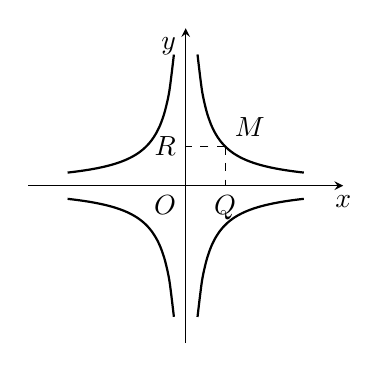
\begin{tikzpicture}[>=stealth, scale=0.5]
		% 1. 绘制坐标轴
		\draw[->] (-4,0) -- (4,0) node[below] {$x$};  % x轴(带箭头和标签)
		\draw[->] (0,-4) -- (0,4) node[below left] {$y$};  % y轴(带箭头和标签)
		\node at (0,0) [below left] {$O$};  % 原点标记
		
		% 2. 绘制双曲线(以 \( xy = 1 \) 和 \( xy = -1 \) 为例,控制“张开程度”)
		% 第一、三象限分支:\( xy = 1 \)
		\draw[thick, domain=0.3:3, smooth, variable=\x] plot (\x, {1/\x});   % 右支
		\draw[thick, domain=-3:-0.3, smooth, variable=\x] plot (\x, {1/\x}); % 左支
		% 第二、四象限分支:\( xy = -1 \)
		\draw[thick, domain=0.3:3, smooth, variable=\x] plot (\x, {-1/\x});  % 右支
		\draw[thick, domain=-3:-0.3, smooth, variable=\x] plot (\x, {-1/\x}); % 左支
		
		% 3. 标记点与辅助线(以 \( M(1,1) \) 为例)
		\coordinate (Q) at (1,0);  % 点Q(x轴上)
		\coordinate (R) at (0,1);  % 点R(y轴上)
		\coordinate (M) at (1,1);  % 点M(双曲线上)
		
		% 绘制虚线辅助线(MQ垂直x轴,MR垂直y轴)
		\draw[dashed] (M) -- (Q);
		\draw[dashed] (M) -- (R);
		
		% 标记点标签
		\node at (Q) [below] {$Q$};
		\node at (R) [left] {$R$};
		\node at (M) [above right] {$M$};
	\end{tikzpicture}
\end{document}
